\xchapter{Seleção e caracterização dos projetos}
{Este capítulo apresenta ...}

A seção \ref{estudo1:introducao} apresenta ...
a seção \ref{estudo1:planejamento} apresenta o planejamento do estudo,
as seções \ref{estudo1:preparacao} e \ref{estudo1:coleta} apresentam detalhes da preparação e execução da coleta de dados,
as seções \ref{estudo1:analise} e \ref{estudo1:interpretacao} apresentam a análise e interpretação dos dados e
a seção \ref{estudo1:conclusoes} apresenta as conclusões do estudo.

% Introduction
% Background
% Experimental Setup (hipoteses / design)
% Results (data analysis)
% Discussion
% Threats to validity
% Conclusions

\section{Introdução e Motivação} \label{estudo1:introducao}

%TROUXE da INTRODUCAO e revisei. PRECISA DE CITACOES.
O software desenvolvido na academia sofre de {\it ``dysfunctional chaotic churn''} [CITAR].
Na prática, isso significa que há muitos projetos com características e funcionalidades parecidas, 
com poucos usuários, com ciclos de vida curtos, e encerrados quando o financiamento inicial termina,
bem como, comunidades desconectadas e paralelas, incompatibilidades entre projetos em um mesmo domínio, 
e tentativas aparentemente não coordenadas de ``reiniciar'' tudo ({\it re-boots}).

\section{Definição} \label{estudo1:definicao} % {{{

% Por que o estudo será realizado?

Sabemos quantos e quais são as características dos projetos de software
acadêmico publicados em conferências de Engenharia de Software?

\subsection{Definição do Objetivo}

\begin{description}
\item{\bf Objeto de estudo.} 
O objeto de estudo são projetos de software de análise estática publicados na literatura acadêmica.

\item{\bf Propósito.} 
O propósito é caracterizar os projetos de software de análise estática desenvolvidos na academia.

\item{\bf Perspectiva.} 
A perspectiva considerada é a de cientistas usuários finais interessados em obter e utilizar software acadêmico.

\item{\bf Foco de qualidade.} 
O principal aspecto de qualidade estudado é a disponibilidade da URL para obtenção do software acadêmico.

\item{\bf Contexto.} 
O estudo foi conduzido com publicações das conferências de Engenharia de Software ASE e SCAM.

\end{description}

\subsection{Sumário da Definição}

%% GQM template

Analisar os \textit{artigos publicados nas conferências de Engenharia de Software ASE e SCAM} % object of study
com o propósito de \textit{encontrar projetos de software acadêmico} % purpose
com respeito a \textit{disponibilidade de URL para obtenção} % quality focus
na perspectiva de \textit{cientistas usuários finais} % perspective
no contexto de \textit{análise estática}. % context

\subsection{Questões de Pesquisa}

Neste estudo as seguintes questões de pesquisa, a respeito
%dos artigos publicados nas conferências ASE e SCAM,
dos projetos de software acadêmico de análise estática publicados nas conferências ASE e SCAM,
serão investigadas:

\newcommand{\EstudoUmQuestaoUm}{Quais são os projetos de software acadêmico de análise estática publicados com identificação de nome e URL?}
\newcommand{\EstudoUmQuestaoDois}{Quantos projetos de software acadêmico de análise estática estão disponíveis para obtenção hoje?}
\newcommand{\EstudoUmQuestaoTres}{Os projetos de software acadêmico de análise estática aceitam explicitamente contribuição de código fonte?}

\begin{description}
  \item [Q1:] \EstudoUmQuestaoUm
  \item [Q2:] \EstudoUmQuestaoDois
  \item [Q2:] \EstudoUmQuestaoTres
\end{description}

\subsection{Métricas}

Para responder às questões de pesquisas, as seguintes métricas serão usadas:

\begin{enumerate}
  \item Número de artigos com publicação de software acadêmico de análise estática com identificação de nome e URL
  \item Número de projetos de software acadêmico de análise estática com URL disponível e acessível
  \item Número de projetos de software acadêmico de análise estática com código fonte disponível e licenciado com permissão de contribuição
\end{enumerate}

% }}} \section{Definição} \label{sec:study1:definition}

\section{Planejamento do Estudo} \label{estudo1:planejamento}

\subsection{Seleção de software acadêmico} % {{{

O contexto deste estudo inclui um conjunto de projetos de software acadêmico ...

\begin{figure}[h]
  \center
  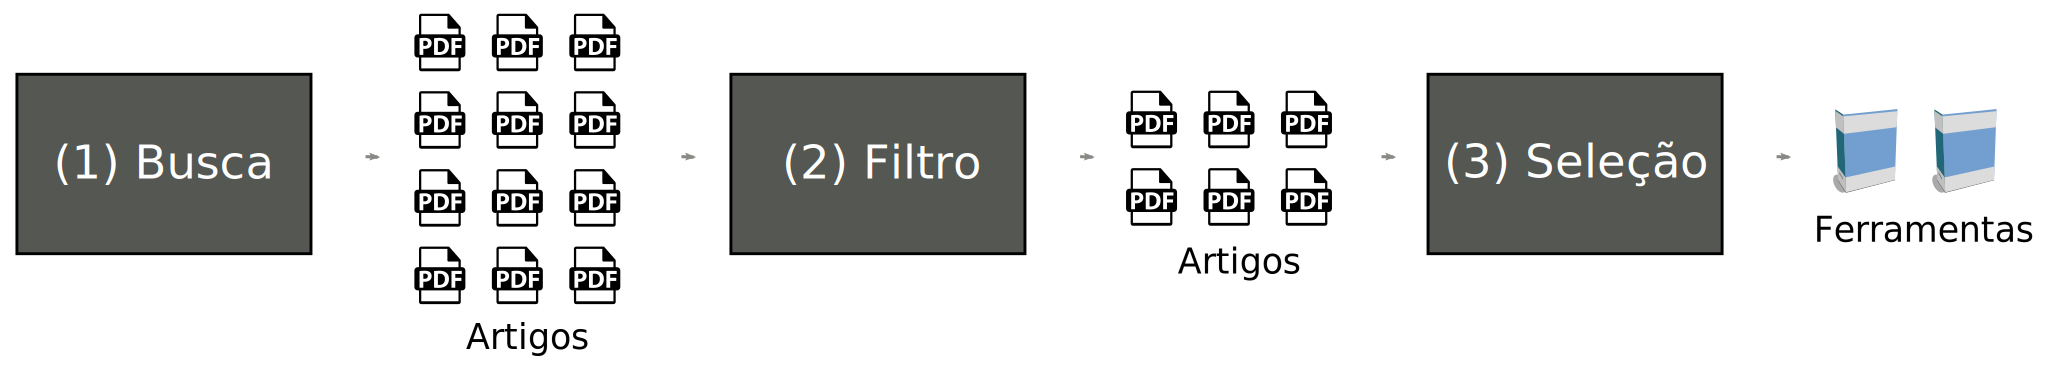
\includegraphics[scale=0.21]{imagens/revisao-estruturada.png}
  \caption{Etapas da seleção de software acadêmico}
  \label{figura-revisao-estruturada}
\end{figure}

A seleção de software acadêmico seguiu um procedimento composto de 3 etapas --
busca, filtro e seleção.
Cada etapa deste procedimento, representada na Figura
\ref{figura-revisao-estruturada}, gera como saída um conjunto de artigos
utilizado como entrada na etapa seguinte.
A última etapa -- seleção -- gera como saída a população de projetos de
software acaêmico de análise estática.

\subsubsection{Busca}

Para a etapa de busca, difinimos as fontes de pesquisa utilizadas como ponto de
partida para selecionar o conjunto inicial de artigos: conferências com
histórico de publicações sobre análise de programas incluindo o maior número de
edições possível.

O resultado da busca são todos copiados localmente em formato pdf e organizados
em diretórios, por conferência e ano de edição.

\subsubsection{Filtro}

%Dos 346 artigos do SCAM e 1533 artigos do ASE analisados na revisão estruturada
%apenas 44\% (155 artigos) e 18\% (281 artigos) continham os termos pesquisados
%no filtro automático da segunda atividade da revisão, respectivamente.

A segunda etapa filtra o conjunto total de artigos através uma busca
textual automática, o objetivo é reduzir o conjunto de artigos inicial,
critérios são aplicados de forma automática em cada artigo do conjunto, se um
artigo não satisfaz um ou mais de um destes critérios ele é excluído do
conjunto final. Cada critério é mapeado num conjunto de strings para
compor a busca final com todos os critérios.

O filtro automático percorre os arquivos pdf de cada artigo, aplicando uma
busca textual em todo o conteúdo, incluindo título, resumo, corpo, referências,
apêndices, anexos e demais seções do arquivo.

\subsubsection{Seleção}

Na etapa de seleção os artigos foram lidos com o principal objetivo
de identificar se entre as contribuições do estudo há menção a software
acadêmico de análise estática, identificado minimamente com nome e URL para
obtenção online. 
Essa leitura foi guiada pelos critérios descritos na Tabela \ref{codes-for-selecao}.

\begin{table}[h]
\caption{Critério for functions \cite{howison2016software}}
\centering
\begin{tabular}{ l p{12cm} }
  \hline
  Código           & Explicação \\
  \hline
  Identificável    & É possível identificar o nome do software acadêmico (ex, Existe um nome, ... "um programa que nós escrevemos?" Podemos encontrar referencias para o software, mesmo que o software não seja encontrado?) \\
  Encontrável      & Uma vez que o software é identificável, podemos encontrar uma fonte online que detalha o software (não necessariamente o próprio software, mas alguma presença oficial) (ex, a página do projeto ou manual online)? \\
  Disponível       & Os autores informam uma URL para obtenção online do software acadêmico \\
%  \item Os autores descrevem o software acadêmico como uma das contribuições do estudo
  \hline
\end{tabular}
\label{codes-for-selecao}
\end{table}

Quando a leitura do título, introdução, resultados e conclusão não foi suficiente
para identificar o software utilizamos as demais seções do artigo. Alguns
artigos descrevem a contribuição de software acadêmico em seções específicas,
por exemplo, é comum o uso de notas de rodapé para indicar URL do projeto de
software acadêmico.

\begin{table}[h]
\caption{Esquema de características coletadas para cada software acadêmico}
\centering
\begin{tabular}{ l p{11cm} }
  \hline
  Característica           & Explicação \\
  \hline
  Nome do software         & O nome do projeto de software \\
  URL                      & Endereço web do software ou projeto, site ou repositório de código fonte, com o software disponível \\
  Título do artigo         & Título do artigo onde o software é citado como contribuição, seja principal ou secundária \\
  Nome do evento           & Nome da conferência onde o software foi publicado \\
  Ano do evento            & Ano da edição da conferência onde o artigo foi publicado \\
  \hline
\end{tabular}
\label{coding-scheme-software-1}
\end{table}

Cada software acadêmico do conjunto foi caracterizado com
as seguintes informações: nome do software, URL do software, título do
artigo, título e ano da confêrencia, como mostra a  Tabela \ref{coding-scheme-software-1}.

% }}} \subsection{Seleção de software acadêmico}

\subsection{Caracterização dos projetos selecionados} % {{{

As informações coletadas pela seleção de projetos foi complementada por meio de
uma pesquisa manual, em diversas fontes: 
artigo original em que o software foi publicado, site do projeto,
repositório de código fonte, manuais e o próprio código fonte, quando disponível.

As informações descritas na Tabela \ref{coding-scheme-software} foram coletadas 
por meio de inspeção manual no website do projeto, de documentos, manuais e artigos.
Quando o código fonte estava disponível, o código fonte foi explorado em busca de 
informações sobre licença, tipo de entrada e linguagens suportadas.

\begin{table}[h]
\caption{Esquema de características coletadas para cada software acadêmico}
\centering
\begin{tabular}{ l p{11cm} }
  \hline
  Característica           & Explicação \\
  \hline
  Descrição do software    & A descrição do projeto de software \\
  Código fonte disponível  & É possível acessar o código fonte de alguma forma? \\
  Acesso                   & Podemos acessar o software agora? Pode receber os seguintes valores: Sem Acesso, Acesso Pago, Acesso Gratuito \\
  Distribuição             & Como o software é distribuído e pode ser acessado? Pode receber os seguintes valores: gratis, foss, proprietário \\
  Licença                  & O software deixa explícito qual licença é distribuído? \\
%  Permissão para modificar & Os criadores dão permissão para modificar o programa (se não menciona modificação, assume não)?; se permissão apenas por contato, também não \\
  Código fonte             & Em qual linguagem de programação o software acadêmico foi desenvolvido \\
  Entradas suportadas      & Qual o tipo de entrada suportada pelo software de análise estática \\
  Linguagens suportadas    & Quais linguagens de programação o software de análise estática suporta como entrada \\
  \hline
\end{tabular}
\label{coding-scheme-software}
\end{table}

Para identificar a linguagem de programação em que o software foi escrito, utilizamos a
ferramenta livre {\it sloccount}\footnote{http://www.dwheeler.com/sloccount}.

% }}} \subsection{Caracterização dos projetos selecionados}

\section{Preparação} \label{estudo1:preparacao}

\subsection{Seleção de software acadêmico} % {{{

\subsubsection{Busca}

Seguindo o planejamento, duas fontes de pesquisa foram utilizadas como ponto de partida para
selecionar o conjunto inicial de artigos: 
%O critério utilizado na definição destas fontes é bastante subjetivo 
%e depende de conhecimento prévio do pesquisador, seus pares, e colaboradores.
a conferência SCAM - {\it Source Code Analysis and
Manipulation Working Conference}\footnote{\url{http://www.ieee-scam.org}} e 
a conferência ASE - {\it Automated Software Engineering}\footnote{\url{http://ase-conferences.org}},
ambas com histórico de publicações sobre análise de programas.
Incluimos todas as edições das duas conferências até o ano de 2015.

\subsubsection{Filtro}

Seguindo o plenajamento definimos os critérios utilizados no filtro deacordo a
Tabela \ref{codes-for-filter}.

\begin{table}[h]
\caption{Critérios para filtro de artigos}
\centering
\begin{tabular}{ l l }
  \hline
  Critério                        & String da busca textual               \\
  \hline
  Menciona software acadêmico     & {\tt tool} ou {\tt framework}         \\
  Disponibiliza online            & {\tt download} ou {\tt available}     \\
  Identifica fonte                & {\tt http} ou {\tt ftp}               \\
  Domínio de análise estática     & {\tt static analysis} ou {\tt parser} \\
  \hline
\end{tabular}
\label{codes-for-filter}
\end{table}

% }}} \subsection{Seleção de software acadêmico}

\subsection{Caracterização dos projetos selecionados} % {{{

Organizamos uma lista de URLs de cada software, criamos para cada projeto uma pasta
no sistema de arquivos onde as informações coletadas serão armazenadas, ...

O software livre {\it sloccount}\footnote{http://www.dwheeler.com/sloccount}
foi instalado.

% }}} \subsection{Caracterização dos projetos selecionados}

\section{Coleta de Dados} \label{estudo1:coleta}

A população estudada compreende um conjunto de 60 projetos de software
acadêmico de análise estática publicados na literatura acadêmica de engenharia
de software.

\subsection{Seleção de software acadêmico} % {{{

A seleção de software acadêmico seguiu um procedimento composto de 3 etapas
conforme descrito no planejamento gerando -- na última etapa de seleção -- a
nossa população de 60 projetos.

\subsubsection{Busca}

A busca resultou em um conjunto inicial de 1873 artigos,
todos copiados localmente em formato pdf e organizados em diretórios, por conferência
e ano de edição.
A Figura \ref{artigos-por-ano} apresenta o total de artigos distribuído
por ano para cada conferência.

\begin{figure}[h]
  \center
  \includegraphics[scale=0.65]{imagens/artigos-por-ano.png}
  \caption{Gráfico em barras com o total de artigos publicado por ano}
  \label{artigos-por-ano}
\end{figure}

\subsubsection{Filtro}

%Dos 346 artigos do SCAM e 1533 artigos do ASE analisados na revisão estruturada
%apenas 44\% (155 artigos) e 18\% (281 artigos) continham os termos pesquisados
%no filtro automático da segunda atividade da revisão, respectivamente.

Ao executar o filtro segundo os critérios definidos na Tabela
\ref{codes-for-filter}, Esta etapa excluiu 1432 artigos do conjunto inicial,
resultando em conjunto, após filtragem, com 441 artigos.

\subsubsection{Seleção}

Na etapa de seleção, os 441 artigos foram lidos,
essa leitura foi guiada pelos critérios descritos na Tabela \ref{codes-for-selecao}.

Encontramos 62 artigos contribuindo com 60 projetos de software acadêmico de
análise estática. O número de projetos de software é menor do que o número
de artigos porque alguns foram mencionados em mais de um artigo. 
%Tabela \ref{coding-scheme-software-1}.

% }}} \subsection{Seleção de software acadêmico}

\subsection{Caracterização dos projetos selecionados} % {{{

As informações coletadas pela seleção de projetos foi complementada por meio de
uma pesquisa manual, em diversas fontes: 
artigo original em que o software foi publicado, site do projeto,
repositório de código fonte, manuais e o próprio código fonte, quando disponível.

As informações descritas na Tabela \ref{coding-scheme-software} foram coletadas 
por meio de inspeção manual no website do projeto, de documentos, manuais e artigos.
Quando o código fonte estava disponível, o código fonte foi explorado em busca de 
informações sobre licença, tipo de entrada e linguagens suportadas.

\begin{table}[h]
\caption{Esquema de características coletadas para cada software acadêmico}
\centering
\begin{tabular}{ l p{11cm} }
  \hline
  Característica           & Explicação \\
  \hline
  Descrição do software    & A descrição do projeto de software \\
  Código fonte disponível  & É possível acessar o código fonte de alguma forma? \\
  Acesso                   & Podemos acessar o software agora? Pode receber os seguintes valores: Sem Acesso, Acesso Pago, Acesso Gratuito \\
  Distribuição             & Como o software é distribuído e pode ser acessado? Pode receber os seguintes valores: gratis, foss, proprietário \\
  Licença                  & O software deixa explícito qual licença é distribuído? \\
%  Permissão para modificar & Os criadores dão permissão para modificar o programa (se não menciona modificação, assume não)?; se permissão apenas por contato, também não \\
  Código fonte             & Em qual linguagem de programação o software acadêmico foi desenvolvido \\
  Entradas suportadas      & Qual o tipo de entrada suportada pelo software de análise estática \\
  Linguagens suportadas    & Quais linguagens de programação o software de análise estática suporta como entrada \\
  \hline
\end{tabular}
\label{coding-scheme-software}
\end{table}

Para identificar a linguagem de programação em que o software foi escrito, utilizamos a
ferramenta livre {\it sloccount}\footnote{http://www.dwheeler.com/sloccount}.

% }}} \subsection{Caracterização dos projetos selecionados}

% \section{Operação} %%%%%%%%

% Raw results from the analysis
\section{Análise dos Dados} \label{estudo1:analise}

Dados de 60 projetos de software acadêmico de análise estática desenvolvidos e
publicados na literatura acadêmica de engenharia de software, informações sobre
diversas formas de menção ao nome destes projetos na literatura acadêmica,
o número de autores mencionando o software ao longo do tempo, informações sobre
lançamentos e novas versões do software, atividade de commits no repositório
de código fonte, informaçoes sobre as formas de distribuição e licenciamento,
dados de acesso ao software.

\input{tab-softwares-data-table.tex}

% Hypothesis rejection
\section{Interpretação dos Resultados} \label{estudo1:interpretacao}

\subsection{Q1 - \EstudoUmQuestaoUm} % {{{

% Demográfica.
Todas as trilhas das duas conferências foram incluídas. 
Encontramos 1873 artigos no total, 1527 artigos do ASE e 346
artigos do SCAM, 
com uma média geral de 75 artigos publicados por ano. 

Até o ano de 1996 a conferencia ASE chamava-se KBSE\footnote{ Knowledge-Based
Software Engineering Conference} e só a partir de 1997 mudou para ASE, a
conferência SCAM teve sua primeira edição apenas em 2001, 10 anos após a
primeira edição do ASE.

No geral, a conferência ASE publica quase 4 vezes mais do que a conferência
SCAM, a edição com o maior número de publicações foi 2011 com 112 artigos
publicados, seguido de 2014 com 104, e 2007 com 102, a edição com o menor
número foi 1996 com apenas 15 artigos publicados.

Detalhes sobre o número de artigos
em cada conferência pode ser consultados nos Apêndices
\ref{artigos-do-scam} e \ref{artigos-do-ase} 

%Situação similar ocorreu com o {\it Augmenting
%Counterexample-Guided Abstraction Refinement with Proof Templates} e o {\it
%PtYasm: Software Model Checking with Proof Templates} publicados no ASE 2008,
%fazem referência ao software PtYasm. 
%Por conta disso, entre os 107 artigos, 

%Ainda durante esta última atividade da revisão cada um dos 107 artigos foram
%analisados em busca de informações sobre onde encontrar o software indicado,

Resultou em 60 softwares com indicação de fonte para obtenção do
software, apenas os artigos que indicam endereço de página web para download do
software foram selecionados, ou seja, uma grande parte dos artigos que produzem
softwares acadêmicos nem ao menos citam o software no paper, ou quando citam,
não informam site ou endereço do projeto para download
\cite{allen2017engineering}, seja código fonte ou apenas binários.

... a Figura \ref{softwares-por-ano} apresenta os resultados distribuídos por ano ...

\begin{figure}[h]
  \center
  \includegraphics[scale=0.65]{imagens/artigos-e-software-por-ano.png}
  \caption{Número total de artigos publicados e publicações com software por ano}
  \label{artigos-e-software-por-ano}
\end{figure}

É possível perceber um crescimento no número de software publicados com o
passar dos anos, de forma que podemos confirmar que considerando as
conferências ASE e SCAM, há um crescimento na publicação de softwares
acadêmicos ao longo do tempo.

Apesar da busca na atividade -- (2) Filtro -- utilizar termos com o objetivo de
encontrar apenas softwares disponíveis com informação de onde encontrar o
software, ainda assim, encontramos 45 artigos com publicação de software sem
indicação de fonte para obtenção.

Entre os 1873 artigos, encontramos 107 artigos referenciando 105 softwares de
análise estática, apenas 60 destes indicam a fonte onde o software pode ser
encontrado.

% }}} Q1

\subsection{Q2 - \EstudoUmQuestaoDois} % {{{

%\citeonline{robles2010replicating} afirma que existe uma tendência das páginas
%web onde os softwares estão disponíveis tem uma grande chance de se tornarem
%indisponíveis ao passar do tempo, investigamos esta tendência 
%cruzando a informação de acesso ao software com a data de publicação do paper
%onde o software foi selecionado.
%a Figura \ref{softwares-disponivel-por-ano} apresenta em cada ano quantos
%porcentos do total de softwares publicados ainda continuam
%disponíveis hoje.

Apenas 37 estão disponíveis, os 23 restantes indicam fonte não mais
acessíveis, endereço não encontrado, indisponível, ou com informações não
relacionadas ao software. 
O Apêndice \ref{resumo-softwares-disponiveis} traz
uma tabela com os nomes e endereços web onde os softwares estão disponíveis.

%Levando em conta a sustentabilidade técnica podemos responder que 
Observamos que 61\% do software acadêmico produzido no domínio de aplicação de análise estática 
são sustentáveis, ou seja, continuam disponíveis ao longo do tempo. 
É importante destacar que não foram considerados aqui artigos que publicaram software 
sem menção à fonte onde o mesmo poderia ser encontrado.
% a revisão estruturada teve como foco encontrar artigos com publicação softwares com indicação de fonte,
% ou seja, aqueles artigos que publicam software mas que não indicam fonte não está sendo
% considerado aqui, vimos que na revisão estruturada, mesmo não sendo o objetivo
Se os artigos que não indicaram a fonte onde o software acadêmico poderia ser encontrado
fossem incluídos -- 45 artigos sem informação de fonte --, 
a taxa de sustentabilidade cairia para apenas 35\%.
Uma revisão estruturada mais abrangente, que desconsiderasse o critério de exclusão
(indicar fonte do software acadêmico), possivelmente resultaria em taxas abaixo dos 35\%, 
sugerindo que a quantidade de software acadêmico publicado em artigos porém indisponível para acesso
pode ser maior do que a encontrada neste estudo.

%TRABALHO FUTURO
%\citeonline{robles2010replicating} afirma que as páginas
%web onde os projetos de software acadêmico foram publicados 
%se tornem indisponíveis com o passar do tempo.
%Podemos investigar esta tendência avaliando os 60 softwares com fonte indicada no artigo,
%identificar se confirmamos neste contexto se com a idade do paper
%as páginas web onde os softwares são publicados tem uma grande chance de se
%tornarem indisponíveis ao passar do tempo.

\begin{figure}[h]
  \center
  \includegraphics[scale=0.65]{imagens/softwares-disponivel-por-ano.png}
  \caption{Gráfico em linha com o total de projetos de software acadêmico disponíveis por ano}
  \label{softwares-disponivel-por-ano}
\end{figure}

A Figura \ref{softwares-disponivel-por-ano} apresenta 
um gráfico em linha com o total de projetos de software acadêmico disponíveis por ano.
Também apresenta a porcentagem de software acadêmico publicado com indicação de fonte que ainda estão
disponíveis, ou seja, a taxa de projetos de software que continuam
disponíveis hoje, considerando o conjunto de projetos de software publicado em cada ano 
com informação sobre fonte para download. 
Os anos de 2002, 2004, 2005, e anteriores a 2001 não possuem software publicado
com fonte indicada no artigo ainda disponível e, portanto,
suas informações não aparecem no gráfico.

Ao analisar a Figura \ref{softwares-disponivel-por-ano},
percebemos que há um leve crescimento na disponibilidade
dos projetos de software acadêmico  nos anos mais recentes.
%
Existe uma leve tendência, ao longo dos anos,  
para a indisponibilidade das fontes informadas e páginas web.
É possível notar que, em 2006, 80\% de todos os
softwares de análise estática publicados nas conferências ASE e SCAM ainda estão disponíveis.
Este número cresce em 2014, chegando a 90\%, e cai no ano seguinte para 85\%.
Apesar de não estar sempre crescente, e da  amostra pequena usada neste estudo 
-- apenas 60 projetos de software acadêmico,
este leve indício confirma a afirmação de \citeonline{robles2010replicating}.

Os 37 softwares com fonte disponível foram avaliados em relação ao segundo
aspecto, isto é, com respeito à forma em que estão disponíveis:
se os artigos informam onde obter tais softwares, se os softwares estão realmente disponíveis, e 
se, ao acessar as fontes indicadas na presente data deste estudo, os softwares estão funcionando e
acessíveis.

Do conjunto de 37 projetos de software estudados, %% Joenio, coloquei aqui o tempo no PRETERITO -- revisar outras partes.
3 não disponibilizaram seu código fonte e  %% Joenio, mudei as frases para VOZ ativa, sujeito: projeto de software.
34 disponibilizaram o código fonte publicamente.
Dentre os que disponibilizaram o código fonte, 13 não informaram licença alguma
%apesar de ter o código fonte disponível, 
e 21 informaram licenças de FOSS ({\it free and open source software}):

\begin{itemize}
  \item 8 usam GNU General Public License;
  \item 2 usam Apache License;
  \item 4 usam BSD License;
  \item 3 usam Eclipse Public License;
  \item 2 usam University of Illinois/NCSA Open Source License;
  \item 1 usa licença {\it FrontEndART Software Ltd}; e
  \item 1 usa licença {\it SAnToS Laboratory Open Academic License}.
\end{itemize}

Entre os 37 softwares disponíveis, 21 podem ser modificados para se adaptar às
necessidades emergentes sem necessidades de solicitação prévia de autorização
aos autores originais devido ao uso de licenças livres. 
Os 13 softwares restantes com código fonte disponível mas sem licença expressa podem
ser modificados, mas a falta de uma licença impõe a necessidade
de solicitar permissão aos autores originais.

35\% dos softwares disponíveis podem ser adaptados de forma incremental para
aproveitar oportunidades emergentes, 21\% podem mediante prévia autorização do
autor original serem modificados, e apenas 5\% não oferecem essa possibilidade
por não disponibilizarem o código fonte publicamente.

%4º Princípio, Persistencia.    % ??????

Os identificadores únicos e metadados descrevendo o software e sua disposição
devem persistir - mesmo além do tempo do software que descrevem.

%Deste total apenas 11\% (41 artigos) e 4\% (62 artigos) foram selecionados na
%terceira e última atividade da revisão contendo publicação de ferramenta de
%análise estática.

%Resultando em 103 artigos com publicação de {\it software científico} de
%análise estática de código fonte, apenas 35 possuem fonte para obtenção do
%software, sendo 32 de código aberto, ou seja, com disponibilidade de
%código fonte, e 3 grátis, apenas binários disponível. Ou seja, apenas 31\% dos
%artigos com publicação de software disponibilizam o código fonte das mesmas.
%Isto significa que 69\% dos artigos com publicação de software de análise
%estática de código fonte são potencialmente impossíveis de serem repetidos, já
%que os artefatos originais são necessários para tal atividade e o artigo não
%disponibiliza o código fonte dos mesmos.

% }}} Q2

\subsection{Q3 - \EstudoUmQuestaoTres} % {{{

Número de menções a cada software acadêmico e qual o contexto e tipo de menção
é feita, quem e quantos são os autores de cada menção.

...

%cada citação pontua no máximo 1 ponto para o peso final do paper ao quanto
%contribui para a sustentabilidade técnica do software, esta pontuação será
%calculada com base nos pesos (em porcentagem) 'contribution\_weight' e
%'authorship\_weight', este último valor é aplicado à contribution weight,
%ou seja contribution\_weight é acrescido a partir do valor de authorship\_weight.
%o valor final se ultrapassar 1 será cortado no limite 1 (máximo), a ideia não é muito
%os números, não queremos saber se são numeros altos, queremos constancia, queremos
%medir se existe um nível de contribuição mínimo aos softwares, isto está
%sendo proposto como algo que mantém o software vivo e útil para a comunidade
%acadêmmica. (por hora o valor mínimo "ideal" por ano é "0.5", ou seja, um
%valor bem modesto, este valor indica que houve ao menos uma contribuição
%ao software, ou que teve citações suficientes equivalente a uma contribuição,
%o software ao ser muito citado ganha mais visibilidade, impacta na possibilidade
%de maior adoção e maior contribuição por terceiros.

% }}} Q3

\subsection{Ameaças à validade}

Validade de construção.
A leitura dos artigos na revisão estruturada para identificar se publicam
softwares de análise estática de código fonte, se disponibilizam fonte para
obtenção de tais softwares, e se os softwares são mesmo do domínio de aplicação
de análise estática de código fonte podem ter maior validade se feitos em
par e revisados por outros pesquisadores.
Neste estudo, estas atividades foram realizadas pelo autor desta dissertação e 
não houve revisão por pesquisadores independentes.
%% A ameaça não foi tratada.

Validade externa. Apenas duas conferências. Apenas duas bases. Apenas um domínio de software acadêmico / uma área do conhecimento em que pesquisadores também programam.
%% A ameaça não foi tratada.

\section{Conclusões} \label{estudo1:conclusoes}

FALTA uma síntese aqui. 
Este estudo ...
Resultados mostram que ...
Algumas tendências emergiram a partir da leitura ...

Planejamos fazer outro estudo ... 
